\section{Task 2}
\label{sec:task2}
As an additional task, we experimented with arbitrary goal poses relative to a 
certain object. 

To this end, we first generated a dataset with the same omniscient controller 
as before, but with random goal poses located in a ring around the object, as 
shown in Figure~\ref{fig:goal-positions}.

\begin{figure}[htbp]
	\centerline{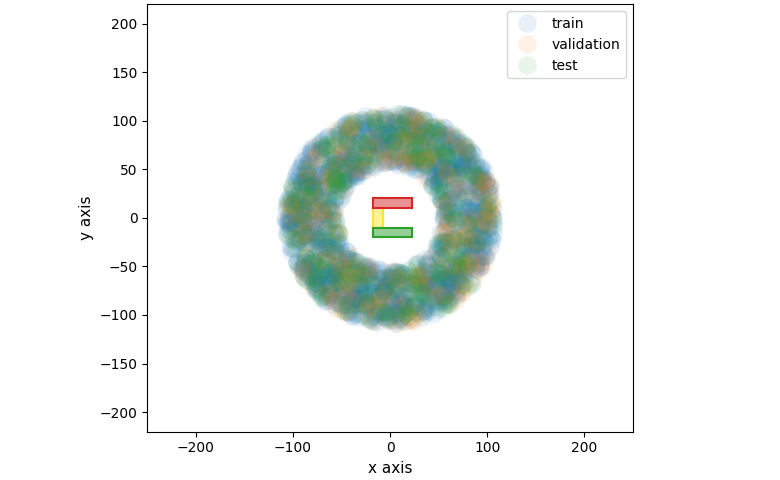
\includegraphics[width=.8\columnwidth]{task2/goal-positions}}
	\caption{Goal positions.}
	\label{fig:goal-positions}
\end{figure}

Then, we implemented a neural network which receives the desired goal pose as 
input to the first fully-connected layer. The architecture used is shown in 
Table~\ref{tab: task 2}.

\begin{table}[htbp]
	\caption{Architecture of the Network for Task 2}
	\begin{center}
		\begin{tabular}{|c|c|c|c|c|}
			\hline
			\textbf{Layer}&\textbf{Channels} &\textbf{Kernel size} 
			&\textbf{Stride} &\textbf{Padding}\\
			\cline{1-5}
			conv1  &  4 $\rightarrow$ 	32 & 5 & 2 & 2, circular \\ \hline
			conv2  & 32 $\rightarrow$  	96 & 5 & 2 & 2, circular \\ \hline
			mpool1 & 					   & 3	& 3 & 1, circular \\ 
			\hline			
			conv3  & 96 $\rightarrow$  	96 & 5 & 1 & 2, circular \\ \hline
			fc1   &  1440 \textbf{+ 3} $\rightarrow$ 128 &  &  &  \\ \hline
			drop1 & \multicolumn{4}{c|}{dropout with p = 0.5} \\ \hline
			fc2   &  128 $\rightarrow$ 128 &  &  &  \\ \hline
			 drop2 & \multicolumn{4}{c|}{ dropout with p = 0.5} \\ \hline
			fc3 &  128 $\rightarrow$   2 &  &  &  \\ \hline
			%\multicolumn{5}{l}{$^{\mathrm{a}}$Sample of a Table footnote.}
		\end{tabular}
		\label{tab: task 2}
	\end{center}
\end{table}

From the plots shown in Figures~\ref{fig:positions-heatmap-2} and 
\ref{fig:goal-reached-2} we can see that the unchanged omniscient controller is 
not perfectly suited for this task: while it was possible to skip collision 
avoidance before, here it results in many runs getting stuck on the object.

\begin{figure}[htbp]
	\centerline{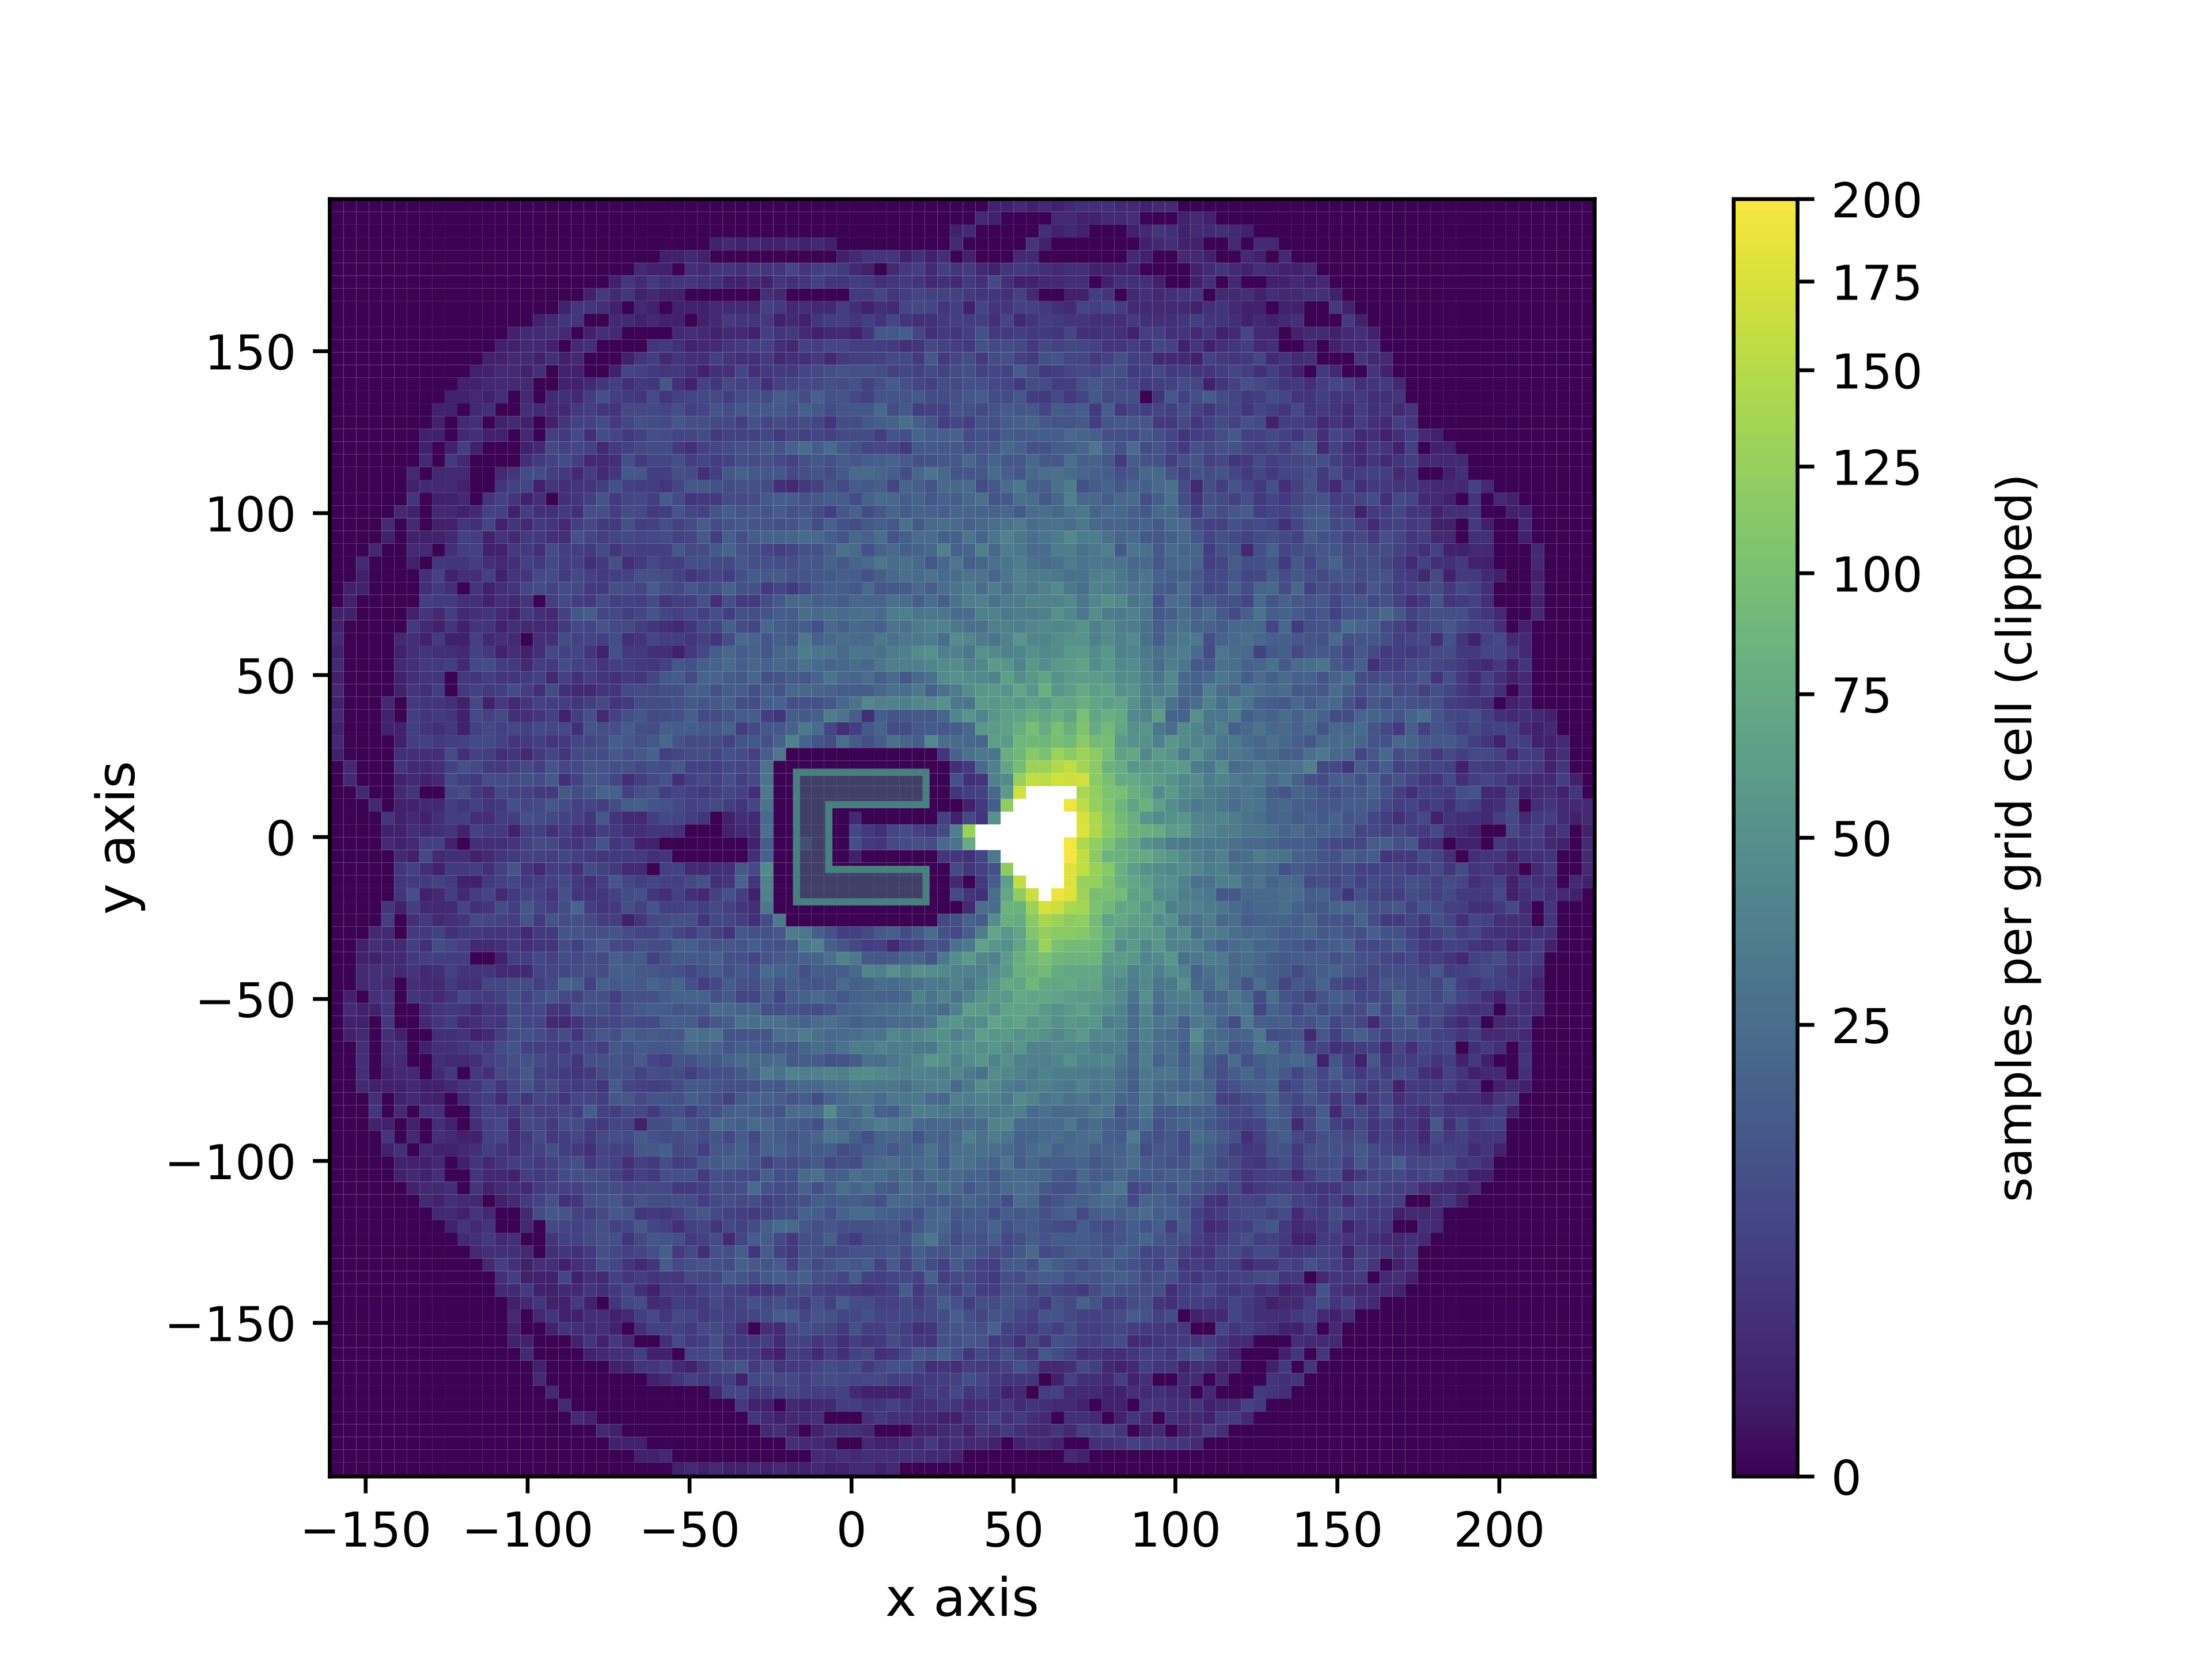
\includegraphics[width=.8\columnwidth]{task2/positions-heatmap}}
	\caption{Positions heatmap.}
	\label{fig:positions-heatmap-2}
\end{figure}

\begin{figure}[htbp]
	\centerline{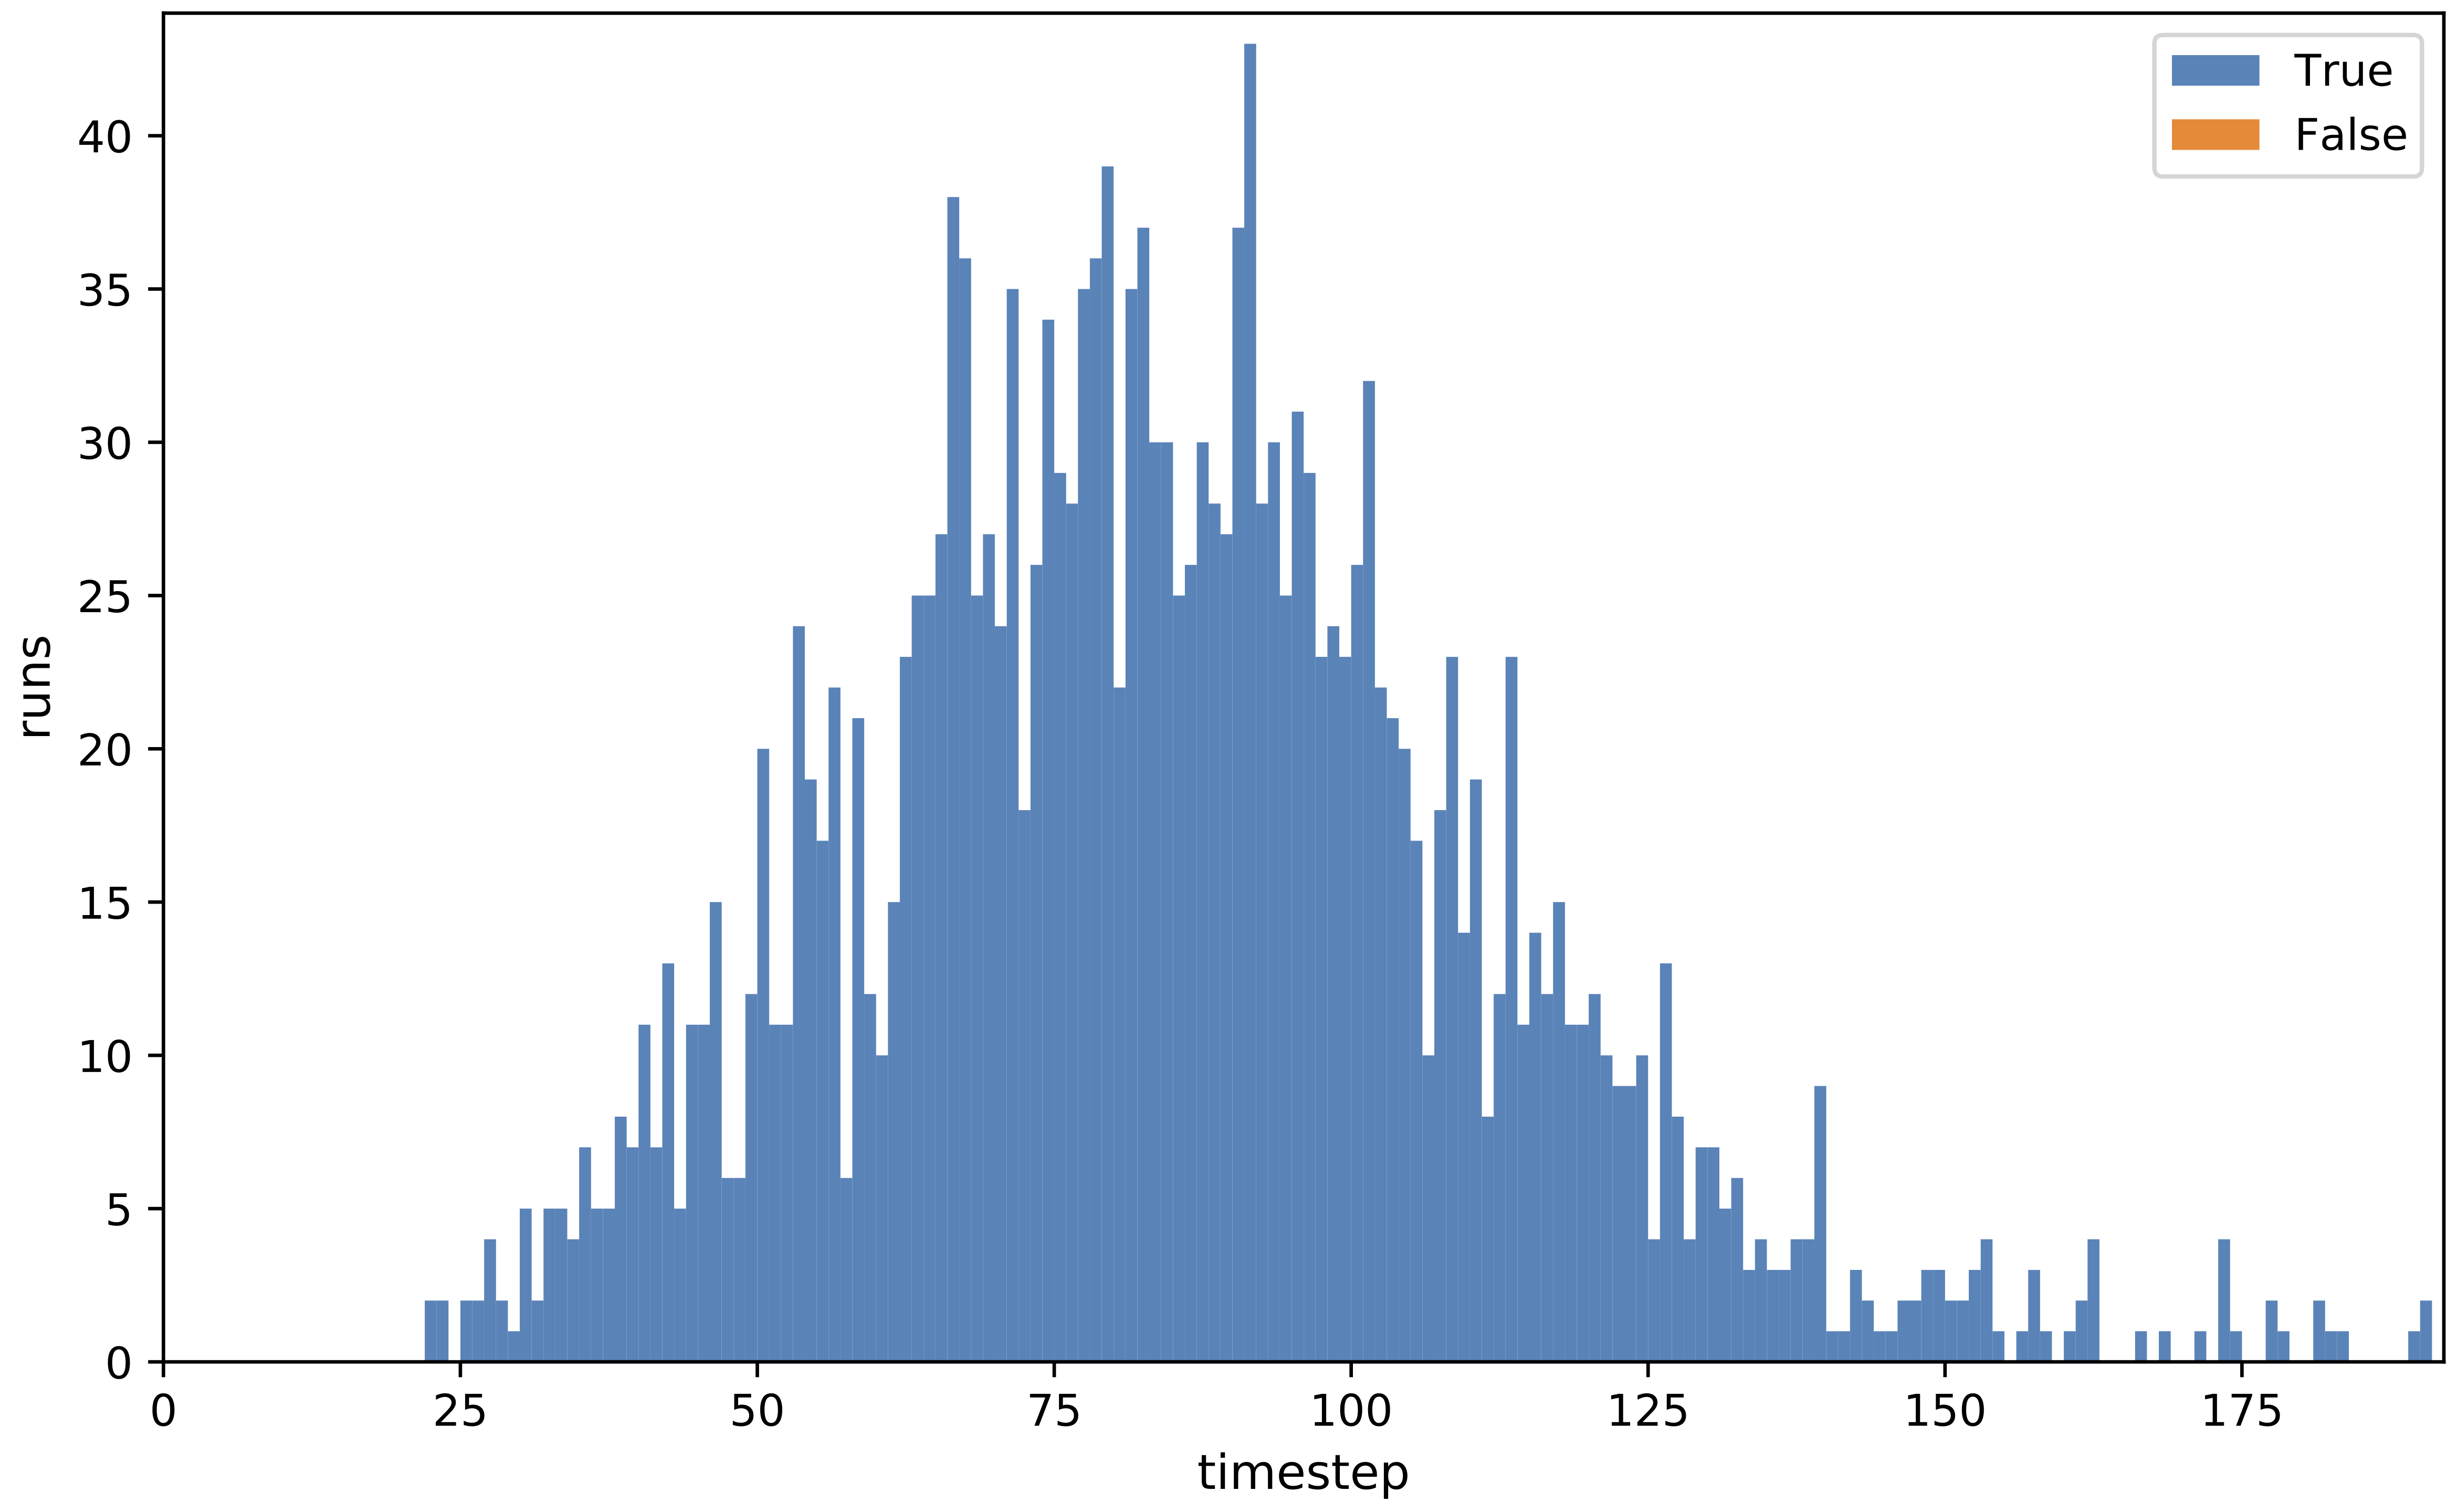
\includegraphics[width=.8\columnwidth]{task2/goal-reached}}
	\caption{Time to reach the goal.}
	\label{fig:goal-reached-2}
\end{figure}

The distances from goal, in Figure~\ref{fig:distances-from-goal-2}, confirm 
this issue, but in general the performance is good when there are no collisions.

\begin{figure}[htbp]
	\centerline{\includegraphics[width=\columnwidth]{task2/distances-from-goal}}
	\caption{Distance from goal.}
	\label{fig:distances-from-goal-2}
\end{figure}

This results in trajectories like those shown in 
Figure~\ref{fig:demo-circle-trajectories-2}.

\begin{figure}[htbp]
	\centerline{\includegraphics[width=\columnwidth]{task2/demo-circle-trajectories}}
	\caption{Trajectories of the controller learned.}
	\label{fig:demo-circle-trajectories-2}
\end{figure}